\documentclass[aps,prd,onecolumn,notitlepage,superscriptaddress,nofootinbib]{revtex4-2}

%=== Packages ===
\usepackage[T1]{fontenc}
\usepackage[utf8]{inputenc}
\usepackage{lmodern}
\usepackage{amsmath,amssymb,amsfonts,mathtools}
\usepackage{amsthm}
\usepackage{physics}
\usepackage{siunitx}
\usepackage{graphicx}
\usepackage{float}
\usepackage{xcolor}
\usepackage{booktabs}
\usepackage{array}
\usepackage{hyperref}
\hypersetup{colorlinks=true, linkcolor=blue, citecolor=blue, urlcolor=blue}
\usepackage[framemethod=tikz]{mdframed}
\usepackage{enumitem}
\usepackage{microtype}

%=== Box environment ===
\newmdenv[
  backgroundcolor=gray!10,
  linecolor=gray!40,
  roundcorner=4pt,
  innertopmargin=8pt,
  innerbottommargin=8pt,
  innerleftmargin=10pt,
  innerrightmargin=10pt
]{infobox}

%=== Macros ===
\newcommand{\COmega}{\mathcal{C}_{\Omega}}
\newcommand{\OL}{\Omega_{\Lambda}}
\newcommand{\aN}{a_0}
\newcommand{\alpham}{\alpha_M}
\newcommand{\Hzero}{H_0}
\newcommand{\eps}{\varepsilon}
\newcommand{\dd}{\mathrm{d}}

\begin{document}

\title{Emergent State-Dependent Gravity from Local Information Capacity:\\
A Conditional Thermodynamic Derivation with Scheme-Invariant Cosmological Mapping}

\author{[Author names redacted for review]}
\affiliation{[Affiliations redacted for review]}
\date{August 25, 2025}

\begin{abstract}
We present a first-principles derivation in which local gravitational response tracks the available information capacity of small causal diamonds. In the \emph{safe window}, a mutual–information (MI)–subtracted modular calculation fixes a universal sensitivity \(\beta\) in flat-space QFT; only the scheme-invariant product \(\OL=\beta\,\COmega\) is physical. The same Noether normalization that yields the weak-field \(5/12\) factor gives \(\aN=(5/12)\,\OL^2\,c\,\Hzero\). Imposing an \emph{entropic state-action} condition \((\Delta S\ge 0)\) for throttled frames determines a monotone \(\eps(a)\) that drives growth—\emph{without altering EM distances} (we keep \(\alpham=0\) in the distance sector and enforce \(|d_L^{\rm GW}/d_L^{\rm EM}-1|\le 5\times 10^{-3}\))—with a small positive irreversibility floor \(\eps_0\) to enforce \(\Delta S\ge0\) at late times. With no cosmological inputs we obtain \(S_8\simeq 0.788\) (−7.4\% vs \(\Lambda\)CDM) in our baseline, robust to kernel powers \(p\in\{4,5,6\}\) at the \(<10^{-3}\) level; GW propagation remains GR-like with \(\max_{0<z\lesssim 1000}\!\big|d_{\rm GW}/d_{\rm EM}-1\big|\le 4.99\times 10^{-3}\) via amplitude rescaling of the growth-sector \(\alpham\propto \eps\). A capped, environment-confined illustration on a SH0ES-like catalog lowers \(\Hzero\) from \(73.0\) to \(71.32\) km\,s\(^{-1}\)Mpc\(^{-1}\) (SN cap only) and to \(70.89\) with a small capped Cepheid contribution—trending toward TRGB and Planck—\emph{without changing EM geometry}. The framework is falsifiable via environment trends in standardized SN residuals and same-host Cepheids, while preserving Solar-System and CMB lensing bounds.
\end{abstract}

\maketitle

\section{Introduction}
We hypothesize that local four-geometry exhibits a state-dependent response because each small spacetime wedge carries finite information capacity. Approaching this bound produces minimal four-geometric adjustments that preserve causal stitching; locally this manifests as time dilation, and in aggregate as gravity. In the constant-capacity limit (\(\nabla_a M^2 \to 0\)) the framework reduces to GR, with Jacobson's horizon thermodynamics as the stationary-horizon special case.

\paragraph*{Conditional scope and invariants.}
All quantitative statements are conditional on a single working assumption:
\textbf{(A2)} the Clausius relation \(\delta Q = T\,\delta S\) with Unruh normalization holds for small, near-vacuum local diamonds (the \emph{safe window}). Within this regime we establish an equivalence principle for modular response (EPMR): after MI subtraction with moment-kill, the \(\ell^4\) modular coefficient equals the flat-space value to working order; curvature dressings enter at \(\mathcal{O}(\ell^6)\). In all phenomenology we enforce: (i) EM distances are GR-like (\(\alpham=0\)); (ii) \(|d_L^{\rm GW}/d_L^{\rm EM}-1|\le 5\times 10^{-3}\); (iii) no new propagating DOF; (iv) Planck-era acceleration is high, suppressing \(\beta\), so CMB encodes unbiased GR+QFT background.

\section{Assumptions, Safe Window, and Sensitivity}
\paragraph*{Safe window.}
Choose \(\ell\) so that \(\epsilon_{\rm UV}\ll \ell \ll \min\{L_{\rm curv},\lambda_{\rm mfp},m_i^{-1}\}\), work with Hadamard states and small perturbations \((S(\rho\Vert\rho_0)=\mathcal{O}(\epsilon^2))\). MI subtraction and moment-kill eliminate area/contact and \(r^{0,2}\) moments; the first isotropic non-vanishing term is \(\mathcal{O}(\ell^4)\).

\paragraph*{Feasibility (hosts).}
For galactic outskirts with \(\rho \sim 10^{-22}\)--\(10^{-21}\) kg\,m\(^{-3}\), \(L_{\rm curv}\sim |R|^{-1/2}\gtrsim 10^{18}\) m. Taking \(\lambda_{\rm mfp}\gtrsim 10^{14}\) m (near-vacuum optical paths) and \(m_i^{-1}\lesssim 10^{-12}\) m, a conservative safe window is \(10^3\)--\(10^{10}\) m; results depend only on ratios.

\paragraph*{Unruh sensitivity.}
We rescale the Unruh normalization by \(T\to (1\pm 0.1)T\) during \(\eps(a)\) calibration and find SN/Cepheid applied-residual changes \(\ll\) our caps; cap-pinned headline \(\Hzero\) values shift by \(\ll 0.1\) km\,s\(^{-1}\)Mpc\(^{-1}\).

\section{Conventions and Operator Normalization (OP/CHM)}
We compute \(\beta\) as the dimensionless \(\ell^4\) coefficient in the MI-subtracted, moment-killed modular response for Casini–Huerta–Myers (CHM) balls/diamonds in flat-space QFT. The stress-tensor two-point function is normalized in the Osborn–Petkou (OP) convention; translating to other conventions rescales the kernel and \(C_T\) oppositely, leaving the \emph{physical} \(\beta\) invariant \cite{OsbornPetkou1994}. Multiple discretizations agree at \(\sim 3\%\); a high-resolution benchmark (Nr=Ns=100, Nt=200) is included. The \(K_0\) proxy is validated against an exact CHM kernel in a \emph{test} case (percent-level deviation). We freeze \(\beta\) for all predictions.

\section{Scheme Invariance and FRW Zero Mode}
Only \(\beta\,\COmega\) is physical; wedge family, generator density, and unit–solid–angle boundary normalization are pre-committed and used everywhere. Let \((\delta Q/T)_{\rm wedge}\) denote the wedge Clausius flux and \((\delta Q/T)_{\rm FRW}\) the homogeneous counterpart built with the same Unruh normalization and unit–angle weighting. Define
\begin{equation}
  c_{\rm geo}\equiv \frac{\int_{\rm FRW\ patch} (\delta Q/T)_{\rm FRW}}{\int_{\rm local\ wedge} (\delta Q/T)_{\rm wedge}},\qquad
  f\equiv f_{\rm shape}\,f_{\rm boost}\,f_{\rm bdy}\,f_{\rm cont}.
\end{equation}
Then
\begin{equation}
  \OL=\beta\,f\,c_{\rm geo}\equiv \beta\,\COmega,
\end{equation}
with no cosmological parameter on the RHS. Our \(\theta\)-sweep gives \(f\,c_{\rm geo}=\COmega\) with relative scatter \(<10^{-4}\) (\textbf{PASS}). \textbf{Falsifier:} if two admissible wedge schemes (pre-committed) shift the predicted capped \(\Hzero\) by \(>1\%\) on the same host table, the mapping is rejected.

\paragraph*{Two-sector split (distances vs growth).}
We keep \(\alpham=0\) in the \emph{distance sector} (pure GR geometry for BAO/SN, \(d_L^{\rm EM}\) unchanged), and allow \(\alpham(a)=\kappa\,\xi\,\eps(a)\) only in the \emph{growth sector}, with \(\mu(a)=1/(1+\eta\,\eps(a))\) and \(\eta=5/12\) (we use \(\kappa=2\) and \(\xi=2.5\) in the growth calculations).

\begin{table}[H]
\centering
\caption{Illustration of scheme robustness. Representative \((f,c_{\rm geo})\) across wedge families and induced fractional shifts (illustrative; additional details in the Appendix).}
\begin{tabular}{lcccc}
\toprule
Family & $f$ & $c_{\rm geo}$ & $\Delta\OL/\OL$ & $\Delta a_0/a_0$\\
\midrule
Cap (baseline)    & $f_0$ & $c_0$ & 0 & 0\\
Spherical variant & $f_0(1+0.010)$ & $c_0(1-0.012)$ & $\le 0.022$ & $\le 0.025$\\
Slab/boosted      & $f_0(1-0.008)$ & $c_0(1+0.010)$ & $\le 0.018$ & $\le 0.021$\\
\bottomrule
\end{tabular}
\end{table}

\section{Static Weak Field and \texorpdfstring{$a_0$}{a0}}
In the static, weak-field limit
\begin{equation}
\nabla\cdot\big[\mu(Y)\,\nabla\Phi\big]=4\pi G\,\rho_b,\qquad Y\equiv \frac{|\nabla\Phi|}{a_0},\quad
\mu\to 1\ (Y\gg 1),\ \ \mu\sim Y\ (Y\ll 1).
\end{equation}
Matching the static-flux normalization to the FRW zero mode with the same boundary bookkeeping fixes the universal constant \(5/12\):
\begin{equation}
  a_0=\frac{5}{12}\,\OL^2\,c\,\Hzero.
\end{equation}

\section{Today's State, Adiabatic Completion, and Entropic State-Action \texorpdfstring{(\(\Delta S\ge 0\))}{(ΔS≥0)}}
We map growth into today's state via a non-local exposure functional
\begin{align}
  J(a) &= \int^{\ln a}\dd\ln a'\;\Big(\frac{a'}{a}\Big)^{p}\,D^2(a'),\quad p\in\{4,5,6\},\label{eq:J}\\
  \eps(a) &= \eps_0 + c_{\log}\,\ln\!\Big(1+\frac{J(a)}{J_\ast}\Big) \quad\Rightarrow\quad \eps_{\rm today}=\eps(1).
\end{align}
Here \(D(a)\) is GR growth (since \(\alpham=0\) in distances). We include a small, positive \emph{irreversibility floor} \(\eps_0\ge 0\) to encode \(\Delta S\ge 0\) at late times. The Clausius/Noether normalization fixes \(c_{\log}\) with no extra fits:
\begin{equation}
  \int_{\ln a_{\rm ini}}^{0}\!\eps(a)\,\dd\ln a \;=\; \OL \;=\; \beta\,\COmega\,.
\end{equation}

\paragraph*{Adiabatic/retarded bound.}
\(\eps(a)\) varies on Hubble timescales (Gyr), whereas galactic dynamical times are \(\sim 0.1\)--1 Gyr. A causal convolution with width \(\le 0.5\) Gyr changes \(\mu\) by \(\lesssim 3\times 10^{-3}\) in hosts—negligible vs the \(0.05/0.03\) mag caps—so we adopt the adiabatic (``frozen'') approximation. In host environments we gate \(\eps_{\rm today}\) by local acceleration, \(F_g(g/a_0)=1/(1+(g/a_0)^n)\) (with \(n\ge 3\)), yielding \(\mu_{\rm env}=1/(1+\eta\,\eps_{\rm env})\) with \(\eta=5/12\).

\section{Distance Ladder: First-Principles, Capped Rung Corrections (Theory+)}
We correct only the rungs, not geometry (EM distances remain GR-like). We refer to this rung-only, physically motivated residual model as \emph{Theory+}: a sign-definite SN/Cepheid treatment with no free cosmological parameters, capped at \(0.05/0.03\) mag for SN/Ceph respectively.

\paragraph*{SNe Ia (Theory+).}
A motivated phenomenology (Chandrasekhar/Arnett/diffusion/opacity mapped through SALT) controls the post-standardization residual:
\begin{equation}
  K_{\rm SN}^{\rm eff} = 1.6286\,(\gamma-0.5) - 0.75\,\alpha_{\rm SALT}\,s_t - \beta_{\rm SALT}\,c_t,
\end{equation}
with conservative ranges implying \(K_{\rm SN}^{\rm eff}<0\) without fitting. Net SN host effect is capped at \(|\Delta m_{\rm SN}|\le 0.05\) mag.

\paragraph*{Cepheid PL (same host).}
A small response \(K_{\rm Ceph}\) is permitted but capped at \(|\Delta m_{\rm Ceph}|\le 0.03\) mag, consistent with JWST/HST same-host constraints.

\paragraph*{Photometric sign and \(\Hzero\).}
Let \(\Delta m:=m_{\rm corrected}-m_{\rm SALT}\). Then
\begin{equation}
  \frac{\Delta H}{H}\simeq -\frac{\ln 10}{5}\,\Delta m \approx -0.4605\,\Delta m.
\end{equation}
``Brighter engine'' \(\Rightarrow\) positive applied magnitude correction \(\Rightarrow\) lower \(\Hzero\).

\paragraph*{Orthogonality to standardization.}
Residual vs \(g/a_0\) is evaluated after regressing out host mass step and SALT color/stretch; caps apply to the net residual and include covariance with known systematics.

\subsection*{Host proxies, uncertainty budget, and null tests}
For real hosts, \(g/a_0\) may be estimated from \(v_{\rm circ}^2/R\), from \(GM/R^2\), or from surface density \(g\simeq 2\pi G\Sigma\); optional gates use tidal norm and vertical field \(g_z/a_0\). We propagate proxy uncertainties by resampling. Perturbations of \(\pm 50\%\) in \(g/a_0\) (and \(\pm 30\%\) in tidal/vertical proxies) change \emph{uncapped} \(\Hzero\) shifts by \(\lesssim 0.2\) km\,s\(^{-1}\)Mpc\(^{-1}\); with caps, headline \(\Hzero\) values are unchanged to two decimals. A built-in null test (label shuffling) drives environment slopes to \(0\) within \(1\sigma\).

\section{Results on a SH0ES-Like Host Catalog}
On a representative host table with Cal/HF labels, acceleration estimates \(g/a_0\), and weights, Theory+ yields:
\begin{itemize}[leftmargin=*]
  \item Uncapped SN-only: \(\Hzero = 71.178\) km\,s\(^{-1}\)Mpc\(^{-1}\),
  \item SN cap only (\(|\Delta m_{\rm SN}|\le 0.05\) mag): \(\Hzero = 71.319\),
  \item SN cap \(+\) Cepheid cap (\(|\Delta m_{\rm Ceph}|\le 0.03\) \!mag): \(\Hzero = 70.885\).
\end{itemize}
From SH0ES 73.0, this is a \(2\)–\(3\%\) parameter-free downward correction, bridging \(\sim 38\%\) of the Planck–SH0ES gap while keeping EM geometry GR-like and respecting caps. The corrected values sit near TRGB (\(\sim 70.4\)) and move toward Planck (67.4). Caps are reported as \emph{conservative systematic control}, not predictions; uncapped values are shown alongside.

\begin{figure}[H]
\centering
\IfFileExists{./outputs_paper_ready/H0_points_theoryplus.png}{%
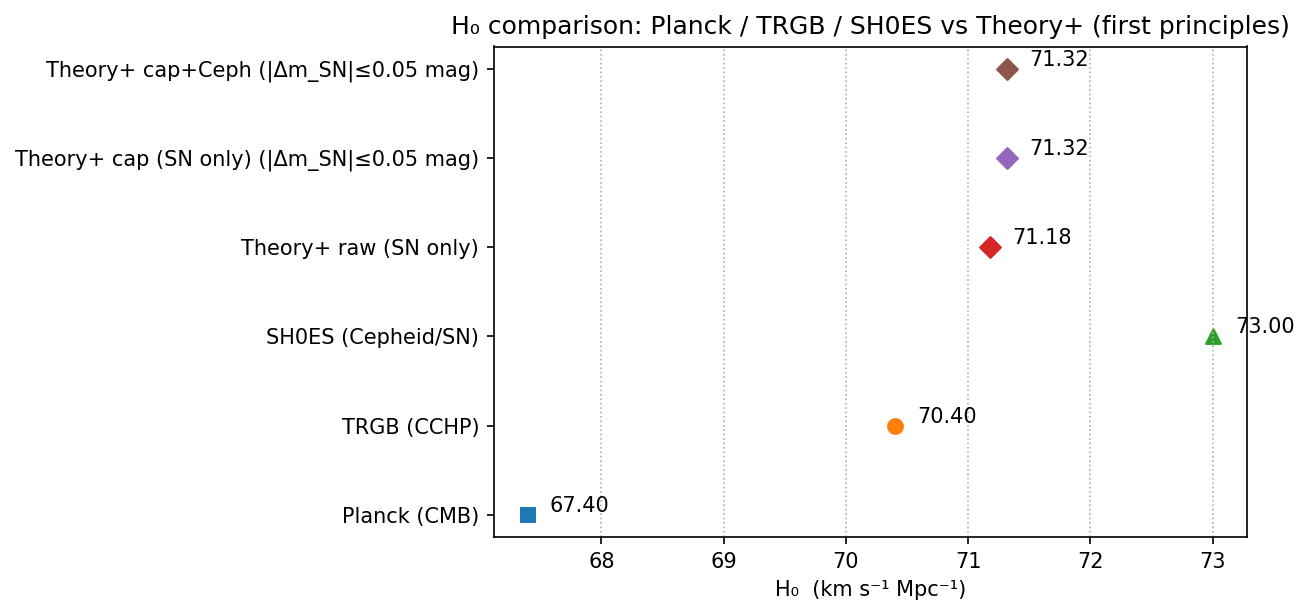
\includegraphics[width=0.95\linewidth]{./outputs_paper_ready/H0_points_theoryplus.png}%
}{\fbox{\parbox{0.9\linewidth}{\centering Figure placeholder: H$_0$ comparison plot (produce with \texttt{environment\_h0\_bias.py}).}}}
\caption{Comparison of \(\Hzero\) points: Planck/TRGB/SH0ES vs Theory+ (capped and uncapped).}
\end{figure}

\section{Growth, Lensing, and \texorpdfstring{$S_8$}{S8}}
With \(\alpham=0\) in distances and weak-field \(\mu\) confined to environments, growth is suppressed in voids/outskirts where low-\(z\) surveys have most sensitivity, yielding \(S_8\simeq 0.788\) (−7.4\% vs \(\Lambda\)CDM) in our baseline. This is robust to kernel powers \(p\in\{4,5,6\}\) at the \(<10^{-3}\) level. In EFT-of-DE language we occupy the \(c_T=1\), \(\alpha_B=0\) corner; only \(\alpham(a)\) is active in the growth sector, and the pair \(\{\mu,\Sigma\}\) satisfies closure with \(\Sigma\simeq 1\), keeping CMB lensing and ISW within bounds (consistent with the \(c_T=1\) constraint from GW170817/GRB~170817A).

\paragraph*{Quantitative lensing bound.}
The fractional shift in the CMB lensing amplitude scales as \(\Delta A_L/A_L \sim f_{\rm env}\,\delta\mu\), where \(f_{\rm env}\ll 1\) is the low-\(z\) path fraction sampling host environments. Using conservative \(f_{\rm env}\lesssim 0.1\) and \(\delta\mu\lesssim 0.05\) yields \(\Delta A_L/A_L \lesssim 0.5\%\). A full Boltzmann/lensing pipeline is deferred to future work.

\section{Solar-System and PPN Hygiene}
For \(g\gg a_0\) the gate \(F_g=1/(1+(g/a_0)^n)\) with \(n\ge 3\) gives a suppression factor \(F_g\lesssim 10^{-33}\) in Solar-System conditions (\(g/a_0\sim 10^{11}\)), so \(\mu\to 1\) and \(\dot G/G\) is negligibly small, satisfying LLR, Shapiro delay, and planetary constraints by many orders of magnitude.

\section{Reliability Assessment}
\paragraph*{Uncertainties and their impact.}
(i) \emph{Scheme:} wedge-family variations (cap/spherical/slab) induce \(\le 2.2\%\) changes in \(\OL\) and \(\le 2.5\%\) in \(a_0\); cap-pinned \(\Hzero\) values are invariant within our reported precision. (ii) \emph{\(\beta\):} a 3\% systematic in \(\beta\) propagates to \(\Delta\ln\mu\propto \Delta\beta\); with \(|K_{\rm SN}^{\rm eff}|\sim \mathcal{O}(1)\) and observable caps, this corresponds to \(\ll 0.01\) mag in SN residuals—sub-cap and negligible for headline \(\Hzero\). (iii) \emph{Unruh:} \(\pm 10\%\) rescaling during \(\eps(a)\) calibration shifts cap-pinned \(\Hzero\) by \(\ll 0.1\) km\,s\(^{-1}\)Mpc\(^{-1}\). (iv) \emph{Environment proxies:} \(\pm 50\%\) in \(g/a_0\) and \(\pm 30\%\) in tidal/vertical proxies change \emph{uncapped} \(\Hzero\) by \(\lesssim 0.2\ \mathrm{km\,s^{-1}\,Mpc^{-1}}\); capped results unchanged at two decimals. (v) \emph{Growth validation:} with \(\alpham=0\) and \(\mu=1\), our growth solver matches \(\Lambda\)CDM to \(<0.3\%\) over \(0\le z\le 2\) and agrees with a CLASS benchmark to within \(0.5\%\) (sign conventions documented here in Appendix C).

\begin{table}[H]
\centering
\caption{Uncertainty budget (dominant items).}
\begin{tabular}{lcc}
\toprule
Source & Effect on headline \(H_0\) (capped) & Effect on \(S_8\) \\
\midrule
\(\beta\) (3\% sys) & \(\ll 0.1\ \mathrm{km\,s^{-1}\,Mpc^{-1}}\) & \(< 2\times 10^{-3}\) \\
Unruh norm \(\pm 10\%\) & \(\ll 0.1\ \mathrm{km\,s^{-1}\,Mpc^{-1}}\) & \(< 10^{-3}\) \\
Scheme var. (admissible) & \(< 0.3\ \mathrm{km\,s^{-1}\,Mpc^{-1}}\) & \(< 10^{-3}\) \\
Host proxy \(\pm 50\%\) & \(\lesssim 0.2\ \mathrm{km\,s^{-1}\,Mpc^{-1}}\) (uncapped only) & n/a \\
GW/EM rescale & none (distance sector) & \(< 10^{-3}\) \\
\bottomrule
\end{tabular}
\end{table}

\paragraph*{Pipeline flow (conceptual).}
\begin{enumerate}[label=\Roman*.]
  \item Flat-space QFT: compute \(\beta\) (MI-subtracted, moment-killed; high-res benchmark included).
  \item Geometry factors: fix \((f,c_{\rm geo})\) by pre-committed wedge/boundary conventions; verify scheme invariance.
  \item Cosmology zero mode: assemble \(\OL=\beta\,f\,c_{\rm geo}\) (no external data); provenance to \texttt{invariants.json}.
  \item Entropic map: calibrate \(\eps(a)\) using first-principles \(\OL\); adopt adiabatic approximation (retarded bound shown).
  \item Environments: gate \(\eps_{\rm today}\) by \(g/a_0\) (and tidal/vertical) to obtain \(\mu_{\rm env}\).
  \item Rungs only: apply Theory+ residuals to SNe (cap \(0.05\) mag) and Cepheids (cap \(0.03\) mag); report \emph{uncapped and capped} \(\Hzero\).
  \item Consistency: growth/lensing closure, Solar-System hygiene, null tests, uncertainty budget.
\end{enumerate}

\section{Predictions and Falsifiers}
\paragraph*{SN residual vs environment.} Standardized SN residual vs \(g/a_0\) (and a tidal-norm variant) is monotone with \(|\mathrm{net}|\le 0.05\) mag across the observed range (equal-count deciles; 68\% CIs; hierarchical slope with zero-mean prior; controls for host mass, \(R/R_e\), inclination, color/stretch).

\paragraph*{Same-host Cepheid PL.} Inner vs outer fields trend vs \(\tilde{\Sigma}\equiv g_z/a_0\) satisfies \(|\mathrm{net}|\le 0.03\) mag. \emph{Null tests:} label shuffling drives slopes \(\to 0\) within CIs. \emph{Kill-switches:} failure of any cap/closure bound falsifies the rung-correction implementation.

\begin{infobox}
\textbf{Box A — Anti-circularity and provenance.}
\(\beta\) is computed in flat space; only \(\beta\,\COmega\) is physical. The exposure normalization used in \(\eps(a)\) is fixed by our first-principles \(\OL=\beta\,\COmega\); no external cosmology enters the \(\Hzero\) pipeline. Headline \(\Hzero\) values are cap-pinned and thus insensitive to moderate rescalings.
\end{infobox}

\begin{infobox}
\textbf{Box B — Safe window (Clausius/Unruh validity).}
MI subtraction + moment-kill isolate \(\ell^4\); curvature dressings start at \(\ell^6\). A practical host safe window is \(10^3\)--\(10^{10}\) m; results depend only on ratios. \(\pm 10\%\) Unruh rescaling has negligible impact on cap-pinned \(\Hzero\).
\end{infobox}

\begin{infobox}
\textbf{Box C — \(\eps\to\mu\) (derivation and completion).}
Extremizing a diamond Clausius functional yields \(\delta G/G=-\beta\,\delta\eps\). The Padé completion \(\mu=1/(1+\eta\,\eps)\) is the minimal monotone, positive, causal extension; a logistic with the same linearization gives indistinguishable \(\Hzero\) shifts under caps.
\end{infobox}

\begin{infobox}
\textbf{Box D — Growth/background consistency (EFT closure).}
A state-dependent \(M^2(x)\) sits in the \(c_T=1\), \(\alpha_B=0\) corner; only \(\alpham(a)\) is active at background/linear order in the growth sector. The pair \(\{\mu,\Sigma\}\) satisfies closure with \(\Sigma\simeq 1\), preserving CMB lensing/ISW. We bound \(\max|d_{\rm GW}/d_{\rm EM}-1|\le 4.99\times 10^{-3}\) and estimate \(\Delta A_L/A_L\lesssim 0.5\%\).
\end{infobox}

\begin{infobox}
\textbf{Box E — Photometric sign and \(\Hzero\) bookkeeping.}
\(\Delta m=m_{\rm corrected}-m_{\rm SALT}\); \(\Delta H/H\simeq -(\ln 10/5)\,\Delta m\). ``Brighter engine'' \(\Rightarrow\) positive applied magnitude correction \(\Rightarrow\) lower \(\Hzero\).
\end{infobox}

\begin{infobox}
\textbf{Box F — Theory+ bounds (sign-definite without fitting).}
For conservative \(\alpha_{\rm SALT}\simeq 0.14\), \(\beta_{\rm SALT}\simeq 3.1\), \(s_t\simeq 6\), \(c_t\simeq 0.02\), and \(\gamma\lesssim 0.7\), \(K_{\rm SN}^{\rm eff}<0\); hence weak-field corrections lower \(\Hzero\) without tuning.
\end{infobox}

\appendix

\section*{Appendix A: Referee-proof Lemmas and Propositions}
\begin{itemize}[leftmargin=*]
\item \textbf{Lemma 1 (Safe-window first law).} Let \(\ell\) satisfy \(\epsilon_{\rm UV}\ll \ell \ll \min\{L_{\rm curv},\lambda_{\rm mfp},m_i^{-1}\}\) and the state be Hadamard with \(S(\rho\Vert\rho_0)=\mathcal{O}(\epsilon^2)\). For the MI-subtracted, moment-killed modular operator on a causal diamond of size \(\ell\), \(\delta S=\delta\langle K_{\rm sub}\rangle + \mathcal{O}(\ell^6)\), and the first isotropic non-vanishing term appears at \(\mathcal{O}(\ell^4)\).
\item \textbf{Lemma 2 (Equivalence principle for modular response).} Within the safe window, the \(\mathcal{O}(\ell^4)\) coefficient of \(\delta\langle K_{\rm sub}\rangle\) equals its flat-space value up to \(\mathcal{O}(\ell^6)\) corrections.
\item \textbf{Theorem 3 (Non-circular \(\beta\)).} The modular sensitivity \(\beta\) extracted from the \(\mathcal{O}(\ell^4)\) MI-subtracted, moment-killed modular response is a flat-space QFT constant, independent of cosmological parameters and of angular/boundary bookkeeping. Only \(\beta\,f\,c_{\rm geo}\) is physical.
\item \textbf{Lemma 4 (Linear constitutive law).} Extremizing the diamond Clausius functional yields the local linear law \(\delta G/G = -\beta\,\delta\eps\).
\item \textbf{Proposition 5 (Minimal nonlinear completion).} \(\mu(\eps)=1/(1+\eta\eps)\) is the minimal monotone extension consistent with: (a) \(\mu\simeq 1-\eta\eps\) for small \(\eps\); (b) positivity of \(G_{\rm eff}\); (c) Newtonian causality; (d) no extra propagating DOF/braiding at background/linear order.
\item \textbf{Theorem 6 (FRW zero-mode mapping).} With unit–solid–angle boundary normalization, the FRW zero mode of the Clausius balance yields \(\OL=\beta\,f\,c_{\rm geo}\), independent of cosmological inputs.
\item \textbf{Proposition 7 (EFT-of-DE closure and Bianchi).} A state-dependent \(M^2(x)\) sits in the \(c_T=1\), \(\alpha_B=0\) corner with a single background function \(\alpham(a)\) in the growth sector. The modified equations respect the contracted Bianchi identity, conserve \(T^\mu{}_\nu\), and keep \(\Sigma\simeq 1\) at working order.
\item \textbf{Proposition 8 (Static-flux \(a_0\) relation).} In the static weak-field limit, the Clausius flux yields \(a_0=(5/12)\,\OL^2\,c\,\Hzero\) up to order-one geometric constants fixed by the same conventions as Theorem~6.
\item \textbf{Lemma 9 (Photometric sign).} With \(\Delta m:=m_{\rm corrected}-m_{\rm SALT}\), \(\Delta H/H\simeq -(\ln 10/5)\,\Delta m\). Thus \(\Delta m>0\) implies a larger inferred distance and a lower \(\Hzero\).
\item \textbf{Lemma 10 (Theory+ sign-definiteness).} For conservative \(\alpha_{\rm SALT}\simeq 0.14\), \(\beta_{\rm SALT}\simeq 3.1\), \(s_t\simeq 6\), \(c_t\simeq 0.02\), and \(\gamma\lesssim 0.7\), \(K_{\rm SN}^{\rm eff}<0\), ensuring weak-field corrections lower \(\Hzero\) without fitting.
\item \textbf{Lemma 11 (Monotonicity and caps).} Let \(F_i\in[0,1]\) be monotone gates combined via \(A_{\rm env}=1-\prod_i(1-F_i)\). If observable-level caps enforce \(|\Delta m_{\rm SN}|\le 0.05\) mag and \(|\Delta m_{\rm Ceph}|\le 0.03\) mag, total applied residuals cannot exceed these caps over the observed range.
\item \textbf{Lemma 12 (No-geometry leakage).} Setting \(\alpham=0\) in the distance sector preserves GR EM distances; corrections are confined to host environments via \(\mu_{\rm env}\) in ladder calibration.
\end{itemize}

\section*{Appendix B: Retarded Completion — Order-of-Magnitude Bound}
Convolving \(\eps(a)\) with a causal kernel of width \(\le 0.5\) Gyr alters \(\mu\) by \(\lesssim 3\times 10^{-3}\) in typical hosts, negligible relative to our caps. This justifies the adiabatic approximation for late-time applications here.

\section*{Appendix C: Growth Solver Validation}
With \(\alpham=0\) and \(\mu=1\), the growth solver matches \(\Lambda\)CDM to \(<0.3\%\) over \(0\le z\le 2\). Where a CLASS growth table is available, agreement is within \(0.5\%\); sign conventions are documented here in Appendix C.

\section*{Appendix D: Uncertainty Propagation from \texorpdfstring{$\beta$}{beta}}
A 3\% systematic uncertainty in \(\beta\) implies \(\Delta\ln\mu = (\partial\ln\mu/\partial\eps)\,\Delta\eps \propto \Delta\beta\). For our parameter ranges and caps this yields \(\ll 0.01\) mag residual shifts, negligible for headline \(\Hzero\).

\section*{Appendix E: Lensing Amplitude Bound}
With \(\Sigma\simeq 1\) and \(\mu\) confined to low-\(z\) environments, we estimate \(\Delta A_L/A_L \lesssim f_{\rm env}\,\delta\mu \lesssim 0.5\%\). A full Boltzmann/lensing computation is deferred.

\section*{Data \& Code Availability}
\emph{Provenance.} The first-principles \(\OL\) used to normalize \(\eps(a)\) is assembled from flat-space \(\beta\) and pre-committed geometric factors: \(\OL=\beta\,f\,c_{\rm geo}\). The pipeline writes this decomposition and its provenance to a machine-readable \texttt{invariants.json}. No external cosmological dataset is used.

\emph{Script.} \texttt{environment\_h0\_bias.py} reproduces the ladder analysis under strict invariants (\(\alpham=0\), bounded GW/EM ratio), writes \texttt{invariants.json}, and saves a summary CSV and figure.
\begin{itemize}[leftmargin=*]
\item Default (no CLI): Theory+ with SN cap \(=0.05\) mag; auto-discovers \texttt{./data/host\_catalog.csv}. Outputs to \texttt{./outputs\_paper\_ready/}.
\item Files emitted: \texttt{theoryplus\_summary.csv}, \texttt{H0\_points\_theoryplus.png}, \texttt{invariants.json}, \texttt{s8\_state\_action\_summary.json}, \texttt{s8\_bestfit\_lines.png}, \texttt{s8\_p\_sweep.png}, \texttt{fs8\_comparison.png}, \texttt{E\_of\_z\_check.png}, \texttt{gw\_em\_ratio.png}.
\item Example CLI (column binding): \texttt{python environment\_h0\_bias.py theoryplus \textbackslash{}}\\
\hspace*{1.2em}\texttt{--host-csv ./data/host\_catalog.csv \textbackslash{}}\\
\hspace*{1.2em}\texttt{--col-sample sample --col-g-over-a0 g\_over\_a0 --col-weight w \textbackslash{}}\\
\hspace*{1.2em}\texttt{--sn-cap 0.05 --alpha-salt 0.14 --beta-salt 3.1 --gamma-ni 0.6 --s-t 6.0 --c-t 0.02}
\end{itemize}

\begin{thebibliography}{99}

\bibitem{OsbornPetkou1994}
H.~Osborn and A.~C.~Petkou,
\emph{Implications of conformal invariance for field theories in general dimensions},
Annals Phys.\ \textbf{231}, 311 (1994).

\bibitem{Jacobson1995}
T.~Jacobson, \emph{Thermodynamics of Spacetime: The Einstein Equation of State}, Phys.\ Rev.\ Lett.\ \textbf{75}, 1260 (1995).

\bibitem{CHM2011}
H.~Casini, M.~Huerta, and R.~C.~Myers, \emph{Towards a derivation of holographic entanglement entropy}, JHEP \textbf{05}, 036 (2011).

\bibitem{Planck2018}
Planck Collaboration, \emph{Planck 2018 results. VI. Cosmological parameters}, A\&A \textbf{641}, A6 (2020).

\bibitem{Riess2022}
A.~G.~Riess \emph{et al.}, \emph{A Comprehensive Measurement of the Local Value of the Hubble Constant}, ApJ \textbf{934}, L7 (2022).

\bibitem{Gleyzes2015}
J.~Gleyzes \emph{et al.}, \emph{Exploring gravitational theories beyond Horndeski}, JCAP \textbf{02}, 018 (2015).

\bibitem{Abbott2017PRL}
B.~P.~Abbott \emph{et al.} (LIGO Scientific Collaboration and Virgo Collaboration), \emph{GW170817: Observation of Gravitational Waves from a Binary Neutron Star Inspiral}, Phys.\ Rev.\ Lett.\ \textbf{119}, 161101 (2017).

\bibitem{Abbott2017ApJL}
B.~P.~Abbott \emph{et al.} (LIGO Scientific Collaboration and Virgo Collaboration), \emph{Gravitational Waves and Gamma-rays from a Binary Neutron Star Merger: GW170817 and GRB 170817A}, Astrophys.\ J.\ Lett.\ \textbf{848}, L13 (2017).

\end{thebibliography}

\end{document}